%% abtex2-modelo-trabalho-academico.tex, v-1.9.2 laurocesar
%% Copyright 2012-2014 by abnTeX2 group at http://abntex2.googlecode.com/ 
%%
%% This work may be distributed and/or modified under the
%% conditions of the LaTeX Project Public License, either version 1.3
%% of this license or (at your option) any later version.
%% The latest version of this license is in
%%   http://www.latex-project.org/lppl.txt
%% and version 1.3 or later is part of all distributions of LaTeX
%% version 2005/12/01 or later.
%%
%% This work has the LPPL maintenance status `maintained'.
%% 
%% The Current Maintainer of this work is the abnTeX2 team, led
%% by Lauro César Araujo. Further information are available on 
%% http://abntex2.googlecode.com/
%%
%% This work consists of the files abntex2-modelo-trabalho-academico.tex,
%% abntex2-modelo-include-comandos and abntex2-modelo-references.bib
%%

% ------------------------------------------------------------------------
% ------------------------------------------------------------------------
% abnTeX2: Modelo de Trabalho Academico (tese de doutorado, dissertacao de
% mestrado e trabalhos monograficos em geral) em conformidade com 
% ABNT NBR 14724:2011: Informacao e documentacao - Trabalhos academicos -
% Apresentacao
% ------------------------------------------------------------------------
% ------------------------------------------------------------------------

\documentclass[
	% -- opções da classe memoir --
	12pt,				% tamanho da fonte
	%openright,			% capítulos começam em pág ímpar (insere página vazia caso preciso)
	oneside,			% para impressão em verso e anverso. Oposto a oneside
	a4paper,			% tamanho do papel. 
	% -- opções da classe abntex2 --
	%chapter=TITLE,		% títulos de capítulos convertidos em letras maiúsculas
	%section=TITLE,		% títulos de seções convertidos em letras maiúsculas
	%subsection=TITLE,	% títulos de subseções convertidos em letras maiúsculas
	%subsubsection=TITLE,% títulos de subsubseções convertidos em letras maiúsculas
	% -- opções do pacote babel --
	english,			% idioma adicional para hifenização
	%french,				% idioma adicional para hifenização
	%spanish,			% idioma adicional para hifenização
	brazil				% o último idioma é o principal do documento
	]{abntex2}

% ---
% Pacotes básicos 
% ---
%\usepackage{lmodern}			% Usa a fonte Latin Modern
\usepackage{times}
\renewcommand*\familydefault{\sfdefault}
\usepackage[T1]{fontenc}		% Selecao de codigos de fonte.
\usepackage[utf8]{inputenc}		% Codificacao do documento (conversão automática dos acentos)
\usepackage{lastpage}			% Usado pela Ficha catalográfica
\usepackage{indentfirst}		% Indenta o primeiro parágrafo de cada seção.
\usepackage{color}				% Controle das cores
\usepackage{graphicx}			% Inclusão de gráficos
\usepackage{microtype} 			% para melhorias de justificação
%\usepackage{type1cm}
% ---
		
% ---
% Pacotes adicionais, usados apenas no âmbito do Modelo Canônico do abnteX2
% ---
%\usepackage{lipsum}				% para geração de dummy text
% ---

% ---
% Pacotes de citações
% ---
%\usepackage[brazilian,hyperpageref]{backref}	 % Paginas com as citações na bibl
\usepackage[alf]{abntex2cite}	% Citações padrão ABNT

% --- 
% CONFIGURAÇÕES DE PACOTES
% --- 

% ---
% Configurações do pacote backref
% Usado sem a opção hyperpageref de backref

% ---

% ---
% Informações de dados para CAPA e FOLHA DE ROSTO
% ---
\titulo{Modularização e Extensão do InteropFrame}
\autor{Felipe Oliveira Carvalho \\ Rodrigo Losano Fontes Calheiros}
\local{São Cristóvão -- SE}
\data{2014}
\orientador{Prof. Dr. Tarcísio da Rocha}
%\coorientador{Equipe \abnTeX}
\instituicao{%
  Universidade Federal de Sergipe -- UFS
  }
\tipotrabalho{Trabalho de Conclusão de Curso}
% O preambulo deve conter o tipo do trabalho, o objetivo, 
% o nome da instituição e a área de concentração 
\preambulo{Pr\'e- Projeto do Trabalho de Conclus\~ao de Curso apresentado como requisito parcial para obten\c c\~ao do t\'itulo de Bacharel em Sistemas de Informa\c{c}\~ao da Universidade Federal de Sergipe.}
% ---


% ---
% Configurações de aparência do PDF final

% alterando o aspecto da cor azul
%\definecolor{blue}{RGB}{41,5,195}

% informações do PDF
%\makeatletter
\hypersetup{
     	%pagebackref=true,
		pdftitle={\@title}, 
		pdfauthor={\@author},
    	pdfsubject={\imprimirpreambulo},
	    pdfcreator={LaTeX with abnTeX2},
		%pdfkeywords={abnt}{latex}{abntex}{abntex2}{trabalho acadêmico}, 
		colorlinks=true,       		% false: boxed links; true: colored links
    	linkcolor=black,          	% color of internal links
    	citecolor=black,        		% color of links to bibliography
    	filecolor=black,      		% color of file links
		urlcolor=black,
		bookmarksdepth=4
}
%\makeatother
% --- 

% --- 
% Espaçamentos entre linhas e parágrafos 
% --- 

% O tamanho do parágrafo é dado por:
\setlength{\parindent}{1.3cm}

% Controle do espaçamento entre um parágrafo e outro:
\setlength{\parskip}{0.2cm}  % tente também \onelineskip

% ---
% compila o indice
% ---
\makeindex
% ---

% ----
% Início do documento
% ----
\begin{document}

% Retira espaço extra obsoleto entre as frases.
\frenchspacing 

% ----------------------------------------------------------
% ELEMENTOS PRÉ-TEXTUAIS
% ----------------------------------------------------------
\pretextual
%Elementos Pré-textuais

%% ---------------------------------------------------------------------------- %
%% CAPA

\thispagestyle{empty}
\begin{titlepage}
    \begin{figure*}
        \centering
        
\includegraphics[keepaspectratio = true, scale=1]{ufs.jpg} \label{fig:logoUFS}
    \end{figure*}
    \vskip 1.5 cm
    \begin{center}
        {\Large UNIVERSIDADE FEDERAL DE SERGIPE \\ CENTRO DE CI\^ENCIAS EXATAS E TECNOL\'OGICAS \\ DEPARTAMENTO DE COMPUTA\c{C}\~AO }\\
        \vspace{6cm}
        {\bf \LARGE Modulariza\c{c}\~ao e Extens\~ao do InteropFrame}\\
        \vspace{3cm}
        {\large Felipe Oliveira Carvalho}\\
				{\large Rodrigo Losano Fontes Calheiros}\\
        \vfill
        \large{S\~ao Crist\'ov\~ao -- SE\\ 2014}
    \end{center}
%\end{titlepage}

%% ---------------------------------------------------------------------------- %
%% Contracapa
%\newpage
%\thispagestyle{empty}
%\onehalfspacing
%\begin{titlepage}
%    \begin{center}
%        {\Large Adonis Vieira de Andrade}\\
%        \vspace{10cm}
%        {\bf \LARGE Aloca\c c\~ao \'O}\\
%        \vfill
%        \large{S\~ao Crist\'ov\~ao -- SE\\ 2013}
%    \end{center}
%\end{titlepage}
%\pagebreak

%% ---------------------------------------------------------------------------- %

% Folha de rosto
\newpage
\thispagestyle{empty}
%\begin{titlepage}
    \begin{center}
        {\Large Felipe Oliveira Carvalho \\ Rodrigo Losano Fontes Calheiros }\\[8.3cm]
        {\LARGE Modulariza\c{c}\~ao e Extens\~ao do InteropFrame} \\[4.3cm]
        \hspace{.45\textwidth} % posicionando a minipage
        \begin{minipage}{.5\textwidth}
            \singlespacing
                Pr\'e- Projeto do Trabalho de Conclus\~ao de Curso apresentado como requisito parcial para obten\c c\~ao do t\'itulo de Bacharel em Sistemas de Informa\c{c}\~ao da Universidade Federal de Sergipe. \\ \\ \\ \\
                
            \onehalfspacing
        \end{minipage}
				{\large Orientador: Prof. Dr. Tarc\'isio da Rocha}
        \vfill
        {\large S\~ao Crist\'ov\~ao -- SE} \\
        {\large 2014}
    \end{center}
%\end{titlepage}
\pagebreak

%-----Folha de aprovação
\newpage
\thispagestyle{empty}
%\begin{titlepage}
    \begin{center}
        {\LARGE Modulariza\c{c}\~ao e Extens\~ao do InteropFrame}\\[2.3cm]
        {\Large Felipe Oliveira Carvalho \\ Rodrigo Losano Fontes Calheiros} \\[1.5cm]
        \hspace{.45\textwidth} % posicionando a minipage
        \begin{minipage}{.5\textwidth}
            \singlespacing
                Pr\'e- Projeto do Trabalho de Conclus\~ao de Curso apresentado como requisito parcial para obten\c c\~ao do t\'itulo de Bacharel em Sistemas de Informa\c{c}\~ao da Universidade Federal de Sergipe. \\

            \onehalfspacing
        \end{minipage}\\[2.5cm]

        \centerline{Aprovado em: \underline{ }\underline{ }\underline{ }\underline{ }\underline{ }\underline{ } /\underline{ }\underline{ }\underline{ }\underline{ }\underline{ }\underline{ } /\underline{ }\underline{ }\underline{ }\underline{ }\underline{ }\underline{ }.}
        \centerline{}
        \centerline{}
        \centerline{Banca Examinadora:}

        \centerline{}
        \centerline{\underline{ }\underline{ }\underline{ }\underline{ }\underline{ }\underline{ }\underline{ }\underline{ }\underline{ }\underline{ }\underline{ }\underline{ }\underline{ }\underline{ }\underline{ }\underline{ }\underline{ }\underline{ }\underline{ }\underline{ }\underline{ }\underline{ }\underline{ }\underline{ }\underline{ }\underline{ }\underline{ }\underline{ }\underline{ }\underline{ }\underline{ }\underline{ }\underline{ }\underline{ }\underline{ }\underline{ }\underline{ }\underline{ }\underline{ }\underline{ }\underline{ }\underline{ }\underline{ }\underline{ }\underline{ }\underline{ }\underline{ }\underline{ }\underline{ }\underline{ }\underline{ }\underline{ }\underline{ }\underline{ }\underline{ }\underline{ }\underline{ }\underline{ }\underline{ }\underline{ }\underline{ }\underline{ }\underline{ }\underline{ }\underline{ }\underline{ }\underline{ }\underline{ }\underline{ }\underline{ }\underline{ }\underline{ }\underline{ }\underline{ }\underline{ }\underline{ }\underline{ }}
        \centerline{Prof. Dr. Tarc\'isio da Rocha (Orientador)}
        \centerline{Universidade Federal de Sergipe}
        \centerline{}

        \centerline{\underline{ }\underline{ }\underline{ }\underline{ }\underline{ }\underline{ }\underline{ }\underline{ }\underline{ }\underline{ }\underline{ }\underline{ }\underline{ }\underline{ }\underline{ }\underline{ }\underline{ }\underline{ }\underline{ }\underline{ }\underline{ }\underline{ }\underline{ }\underline{ }\underline{ }\underline{ }\underline{ }\underline{ }\underline{ }\underline{ }\underline{ }\underline{ }\underline{ }\underline{ }\underline{ }\underline{ }\underline{ }\underline{ }\underline{ }\underline{ }\underline{ }\underline{ }\underline{ }\underline{ }\underline{ }\underline{ }\underline{ }\underline{ }\underline{ }\underline{ }\underline{ }\underline{ }\underline{ }\underline{ }\underline{ }\underline{ }\underline{ }\underline{ }\underline{ }\underline{ }\underline{ }\underline{ }\underline{ }\underline{ }\underline{ }\underline{ }\underline{ }\underline{ }\underline{ }\underline{ }\underline{ }\underline{ }\underline{ }\underline{ }\underline{ }\underline{ }\underline{ }}
        \centerline{Prof. xxxxx xxxxxxx xxxxxxx}
        \centerline{Universidade Federal de Sergipe}
        \centerline{}

        \centerline{\underline{ }\underline{ }\underline{ }\underline{ }\underline{ }\underline{ }\underline{ }\underline{ }\underline{ }\underline{ }\underline{ }\underline{ }\underline{ }\underline{ }\underline{ }\underline{ }\underline{ }\underline{ }\underline{ }\underline{ }\underline{ }\underline{ }\underline{ }\underline{ }\underline{ }\underline{ }\underline{ }\underline{ }\underline{ }\underline{ }\underline{ }\underline{ }\underline{ }\underline{ }\underline{ }\underline{ }\underline{ }\underline{ }\underline{ }\underline{ }\underline{ }\underline{ }\underline{ }\underline{ }\underline{ }\underline{ }\underline{ }\underline{ }\underline{ }\underline{ }\underline{ }\underline{ }\underline{ }\underline{ }\underline{ }\underline{ }\underline{ }\underline{ }\underline{ }\underline{ }\underline{ }\underline{ }\underline{ }\underline{ }\underline{ }\underline{ }\underline{ }\underline{ }\underline{ }\underline{ }\underline{ }\underline{ }\underline{ }\underline{ }\underline{ }\underline{ }\underline{ }}
        \centerline{Prof. xxxxxx xxxxxxx xxxxxx}
        \centerline{Universidade Federal de Sergipe}
        \centerline{}

        \vfill
        {\large S\~ao Crist\'ov\~ao -- SE} \\
        {\large 2014}
    \end{center}
\end{titlepage}
\pagebreak

%-----FIm da folha de aprovação


%\pagenumbering{roman}     % começamos a numerar

% ---------------------------------------------------------------------------- %
% Agradecimentos:
% Se o candidato não quer fazer agradecimentos, deve simplesmente eliminar esta página

%\chapter*{Agradecimentos}
%
%Agrade\c co aos meus pais pela oportunidade que me deram de estudar e pelo carinho e apoio em todos os momentos.
%
%\`A minha namorada, Monique, por todo o incentivo e apoio nas horas dif\'iceis.
%
%Aos meus amigos, em especial a turma 2007, pela amizade e companheirismo durante todos esses anos.
%
%Ao meu orientador Professor \^Angelo M. F. de Almeida pelo tempo disponibilizado para me ajudar e guiar ao longo deste trabalho.

% ---------------------------------------------------------------------------- %

% Resumo
%\chapter*{Resumo}

%O desenvolvimento de Sistemas Distribu\'idos tem se tornado uma tarefa complexa. Uma t\'ecnica que tornou-se amplamente utilizada no desenvolvimento desses sistemas \'e a Engenharia de Software Baseada em Componentes (ESBC), o que resultou no surgimento de diversos modelos de componentes. Um desafio que surge do desenvolvimento baseado em componentes \'e o da interoperabilidade entre partes heterog\^eneas desenvolvidas em diferentes modelos de componentes. Em geral, o problema da interoperabilidade entre partes heterog\^eneas de um sistema \'e tratado pelo uso de \textit{middlewares}. Sistemas de \textit{middleware} s\~ao capazes de promover integra\c{c}\~ao e abstrair do desenvolvedor detalhes dessa integra\c{c}\~ao.

%Dentro desse contexto foi criado o InteropFrame, um \textit{middleware} que lida com a interoperabilidade entre sistemas distribu\'idos desenvolvidos nos modelos de componentes OpenCOM e Fractal, al\'em de tratar de detalhes de comunica\c{c}\~ao remota utilizando RMI e \textit{Web Services SOAP}. O InteropFrame \'e uma solu\c{c}\~ao desenvolvida em Java puro e \'e extens\'ivel para o suporte a novos modelos de componentes e tamb\'em de comunica\c{c}\~ao remota. Por\'em, por ser desenvolvido em Java puro, esse suporte fica dificultado, uma vez que n\~ao s\~ao estabelecidas interfaces modulares para a extensibilidade. Al\'em dessa problem\'atica, o InteropFrame tamb\'em possui limita\c{c}\~oes na comunica\c{c}\~ao remota interna.

%Este trabalho prop\~oe a modulariza\c{c}\~ao do InteropFrame utilizando o modelo OSGi, de forma a reorganizar sua arquitetura em \textit{plug-ins} para os modelos de componentes suportados e tamb\'em para os modelos de comunica\c{c}\~ao remota. Visando confirmar a proposta de modulariza\c{c}\~ao, ser\'a adicionado o suporte ao modelo OSGi para tornar-se interoper\'avel com os modelos j\'a suportados pelo InteropFrame. Al\'em da modulariza\c{c}\~ao, ser\~ao feitas melhorias internas na comunica\c{c}\~ao remota do InteropFrame.
%\newline
%\newline
%\noindent \textbf{Palavras-chave:} Modelos de Componentes, Interoperabilidade, Modulariza\c{c}\~ao, Sistemas Distribu\'idos.

% ---------------------------------------------------------------------------- %
% Abstract
%\chapter*{Abstract}
%
%This paper deals with the optimal allocation of telecontrolled switches and its main advantages in a distribution system feeder. This problem is solved using a Genetic Algorithm which has as its fitness function minimize the losses by energy not supplied. A real feeder is modeled and its continuity index are calculated using a logical structural matrix. The load flow calculation is made by applying the Power Summation Method. The implemented Genetic Algorithm is validated through the allocation of 2 telecontrolled switches in a real distribution system feeder. Advantages of allocation of 2 and 3 telecontrolled switches are compared and analyzed between themselves.
%\\
%
%\noindent \textbf{Keywords:} Genetic Algorithm,optimal allocation of telecontrolled switches, Distribution System  .

% ---------------------------------------------------------------------------- %
% Sumário
%\tableofcontents    % imprime o sumário

%%% ---------------------------------------------------------------------------- %
%\chapter{Lista de Abreviaturas}
%\begin{tabular}{ll}

%IDE & Integrated Development Enviroment \\
%OSGi & Open Services Gateway Initiative \\
%XML & Extensible Markup Language \\		 
   
%\end{tabular}

% ---------------------------------------------------------------------------- %


% Listas de figuras e tabelas criadas automaticamente
%\listoffigures
%\listoftables



% ---
% Capa
% ---
%\imprimircapa
% ---

% ---
% Folha de rosto
% (o * indica que haverá a ficha bibliográfica)
% ---
%\imprimirfolhaderosto*
% ---

% ---
% Inserir a ficha bibliografica
% ---

% Isto é um exemplo de Ficha Catalográfica, ou ``Dados internacionais de
% catalogação-na-publicação''. Você pode utilizar este modelo como referência. 
% Porém, provavelmente a biblioteca da sua universidade lhe fornecerá um PDF
% com a ficha catalográfica definitiva após a defesa do trabalho. Quando estiver
% com o documento, salve-o como PDF no diretório do seu projeto e substitua todo
% o conteúdo de implementação deste arquivo pelo comando abaixo:
%
% \begin{fichacatalografica}
%     \includepdf{fig_ficha_catalografica.pdf}
% \end{fichacatalografica}

% ---

% ---
% Inserir errata
% ---

% ---

% ---
% Inserir folha de aprovação
% ---

% Isto é um exemplo de Folha de aprovação, elemento obrigatório da NBR
% 14724/2011 (seção 4.2.1.3). Você pode utilizar este modelo até a aprovação
% do trabalho. Após isso, substitua todo o conteúdo deste arquivo por uma
% imagem da página assinada pela banca com o comando abaixo:
%
% \includepdf{folhadeaprovacao_final.pdf}
%

% ---
\pagenumbering{roman}
% ---
% Dedicatória
% ---

% ---

% ---
% Agradecimentos
% ---

% ---

% ---
% Epígrafe
% ---

% ---

% ---
% RESUMOS
% ---

% resumo em português
\setlength{\absparsep}{18pt} % ajusta o espaçamento dos parágrafos do resumo
\begin{resumo}
 O desenvolvimento de Sistemas Distribu\'idos tem se tornado uma tarefa complexa. Uma t\'ecnica que tornou-se amplamente utilizada no desenvolvimento desses sistemas \'e a Engenharia de Software Baseada em Componentes (ESBC), o que resultou no surgimento de diversos modelos de componentes. Um desafio que surge do desenvolvimento baseado em componentes \'e o da interoperabilidade entre partes heterog\^eneas desenvolvidas em diferentes modelos de componentes. Em geral, o problema da interoperabilidade entre partes heterog\^eneas de um sistema \'e tratado pelo uso de \textit{middlewares}. Sistemas de \textit{middleware} s\~ao capazes de promover integra\c{c}\~ao e abstrair do desenvolvedor detalhes dessa integra\c{c}\~ao.

Dentro desse contexto foi criado o InteropFrame, um \textit{middleware} que lida com a interoperabilidade entre sistemas distribu\'idos desenvolvidos nos modelos de componentes OpenCOM e Fractal, al\'em de tratar de detalhes de comunica\c{c}\~ao remota utilizando RMI e \textit{Web Services SOAP}. O InteropFrame \'e uma solu\c{c}\~ao desenvolvida em Java puro e \'e extens\'ivel para o suporte a novos modelos de componentes e tamb\'em de comunica\c{c}\~ao remota. Por\'em, por ser desenvolvido em Java puro, esse suporte fica dificultado, uma vez que n\~ao s\~ao estabelecidas interfaces modulares para a extensibilidade. Al\'em dessa problem\'atica, o InteropFrame tamb\'em possui limita\c{c}\~oes na comunica\c{c}\~ao remota interna.

Este trabalho prop\~oe a modulariza\c{c}\~ao do InteropFrame utilizando o modelo OSGi, de forma a reorganizar sua arquitetura em \textit{plug-ins} para os modelos de componentes suportados e tamb\'em para os modelos de comunica\c{c}\~ao remota. Visando confirmar a proposta de modulariza\c{c}\~ao, ser\'a adicionado o suporte ao modelo OSGi para tornar-se interoper\'avel com os modelos j\'a suportados pelo InteropFrame. Al\'em da modulariza\c{c}\~ao, ser\~ao feitas melhorias internas na comunica\c{c}\~ao remota do InteropFrame.

 \textbf{Palavras-chaves}: Modelos de Componentes, Interoperabilidade, Modulariza\c{c}\~ao, Sistemas Distribu\'idos.
\end{resumo}

% resumo em inglês
\begin{resumo}[Abstract]
 \begin{otherlanguage*}{english}
   This is the english abstract.

   \vspace{\onelineskip}
 
   \noindent 
   \textbf{Key-words}: Component Models, Interoperability, Modularization, Distributed Systems.
 \end{otherlanguage*}
\end{resumo}

% ---

% ---
% inserir lista de ilustrações
% ---

% ---

% ---
% inserir lista de tabelas
% ---

% ---

% ---
% inserir lista de abreviaturas e siglas
% ---

% ---

% ---
% inserir lista de símbolos
% ---

% ---

% ---
% inserir o sumario
% ---
\pdfbookmark[0]{\contentsname}{toc}
\tableofcontents*
\cleardoublepage
% ---



% ----------------------------------------------------------
% ELEMENTOS TEXTUAIS
% ----------------------------------------------------------
\textual
\inputencoding{latin1}
\setcounter{page}{1}
\pagenumbering{arabic}
\chapter{Introdu��o}\label{chap:introducao}

\section{Considera��es Iniciais} \label{sec.consideracos_iniciais}

Um sistema distribu�do � considerado aquele no qual os componentes localizados em computadores interligados em rede se comunicam e coordenam suas a��es apenas passando mensagens. (COLOURIUS, 2007). Tem como objetivo adicionar o poder computacional de diversos computadores, interligados por uma rede, para compartilhar a execu��o de tarefas.

O desenvolvimento de sistemas para este ambiente tem se tornado uma tarefa complexa, e como o n�mero de recursos exigidos em sistemas distribu�dos � crescente isso faz com que a complexidade no desenvolvimento dos sistemas aumente (Blair et al. 2011).  Uma abordagem utilizada para lidar com esse problema � o desenvolvimento baseado em componentes, que permite desenvolver software atrav�s da composi��o de componentes individuais com prop�sitos bem definidos, possibilitando aumentar a produtividade, reusabilidade e manutenabilidade do software.

O uso da abordagem do desenvolvimento baseado em componentes traz consigo alguns problemas, como: a exist�ncia de in�meros modelos diferentes de componentes para sistemas distribu�dos, onde cada modelo possui sua especificidade do c�digo t�cnico para o desenvolvimento de componentes e seu pr�prio padr�o de desenvolvimento. O que exige do desenvolvedor o conhecimento especifico de caracter�sticas de cada modelo. Devido a diversidade de modelos a reusabilidade de componentes de software de modelos distintos � dificultada, uma vez que n�o h� uma interoperabilidade nativa entre modelos de componentes heterog�neos.

Para minimizar os problemas apresentados quanto ao desenvolvimento de sistemas distribu�dos baseados em componentes, um framework para desenvolvimento em alto n�vel foi proposto em (SANTOS; ROCHA, 2013). Este framework visa disponibilizar um modelo de programa��o gen�rico que � fornecido ao desenvolvedor atrav�s de anota��es no c�digo de neg�cio da aplica��o. Assim, componentes de modelos espec�ficos s�o gerados a partir destas anota��es, solu��o que livra o desenvolvedor de ter que conhecer detalhes t�cnicos de cada modelo que se deseja utilizar. Al�m disso, este framework retira do desenvolvedor a necessidade de conhecer m�todos de comunica��o remota distribu�da, tratando a complexidade de desenvolvimento de objetos distribu�dos. Chamado de HighFrame, ele � composto por um reposit�rio, que fica situado em um servidor, que cont�m todos os componentes gen�ricos possibilitando assim a reutiliza��o dos mesmos por diversos usu�rios; e por um Planejador Gr�fico, que � a ferramenta na qual o desenvolvedor pode compor a arquitetura do sistema distribu�do em alto n�vel.

O framework destacado anteriormente apresenta um conjunto de recursos para minimizar a complexidade de desenvolvimento de sistemas distribu�dos baseados em compoenentes. Por�m, esta solu��o para desenvolvimento n�o apresentou a implementa��o de planejador gr�fico da arquitetura para fornecer alto n�vel no desenvolvimento de sistemas distribu�dos. Assim, entendendo que uma ferramenta gr�fica � um m�dulo de fundamental import�ncia para o fornecimento do alto n�vel no framework, este trabalho prop�e um Planejador Gr�fico de arquitetura de sistemas distribu�dos baseados em componentes.


%\section{Revis�o Bibliogr�fica} \label{sec.rev_bibliografica}

 

\section{Objetivos do Trabalho}

Estudar, modelar e implementar um Planejador Gr�fico para o desenvolvimento em alto n�vel de sistemas distribu�dos baseado em componentes.

\subsection{Objetivo Geral}
Este trabalho tem como objetivo principal o desenvolvimento de uma IDE para o planejamento em alto n�vel da Arquitetura de sistemas distribu�dos baseados em componentes gen�ricos especificados pela HighFrame framework.

\subsection{Objetivos Espec�ficos}
\begin{itemize}
  \item  Estudo do HighFrame framework;
  \item  Levantamento dos requisitos da aplica��o a ser desenvolvida;
  \item  Modelagem;
	\item  Implementa��o; e
	\item Cria��o do Manual de Uso.
\end{itemize}


\section{Organiza��o do Trabalho}

No cap�tulo 2 � apresentada a fundamenta��o te�rica necess�ria dos temas relacionados com o desenvolivmento da solu��o.
No cap�tulo 3 ser� apresentado o HighFrame Designer, detalhando a modelagem e implementa��o.
No cap�tulo 4 ser� apresentado o Manual de uso da ferramenta.
No cap�tulo 5 a Conclus�o.





\chapter{Fundamenta��o}\label{chap:fundamentacao}

Esta se��o apresenta os fundamentos necess�rios para o entendimento da solu��o. Assim como apresenta uma breve descri��o de IDEs existentes com suas qualidades e limita��es.

\section{Desenvolvimento Baseado em Componentes} \label{sec.desvol_comp}

	
Para se tentar resolver a crescente dificuldade em se desenvolver softwares existem v�rios processos, sendo um deles o de dividir o desenvolvimento em partes menores. Partindo dessa ideia foi criado o conceito de componentes de software.

A Engenharia de Software Baseada em Componentes apresenta-se como um dos elementos chave na constru��o de middlewares e sistemas distribu�dos. Flexibilidade e reusabilidade s�o algumas das principais vantagens na utiliza��o de componentes, frameworks de componentes possibilitam que componentes sejam modificados ou substitu�dos em tempo de execu��o, garantindo assim a disponibilidade do sistema.

\subsection{Elementos da Arquietura Baseada em Componentes}

A arquitetura baseada em componentes tem como elementos b�sicos: componentes, interfaces e contratos. 

Componentes s�o definidos por (SZYPERSKI et al, 2008) como sendo unidades de composi��o com interfaces contratualmente especificadas e depend�ncias de contexto explicitas, que podem ser implantados de maneira independente e est�o sujeitos a composi��o por terceiros.

Interfaces de componentes podem ser definidas como sendo uma especifica��o do seu ponto de acesso, ou seja, os clientes acessam por eles os servi�os providos por um componente. N�o contem nenhuma implementa��o e sim a listagem das opera��es e as descri��es e os protocolos destas opera��es. Isso torna poss�vel que se fa�a uma mudan�a somente na implementa��o sem que seja preciso alterar a sua interface e que sejam adicionadas novas interfaces sem que seja preciso modificar a implementa��o j� existente do componente. Podem ser de dois tipos: providas e requeridas, que basicamente significa que a primeira especifica os servi�os oferecidos pelo componente enquanto que a segunda os servi�os requeridos pelo mesmo.

Os contratos listam as restri��es globais que os componentes ter�o, e tamb�m lista as pr� e p�s condi��es que precisam ser preenchidas para cada opera��o existente no componente. Isto pode ser considerado como sendo o comportamento de um componente. Servem tamb�m para definir o comportamento de um grupo de componentes que interagem entre si.

\subsection{\textit{Framework} de Componentes}

Um framework pode ser entendido como sendo um conjunto de classes que colaboram para realizar uma responsabilidade para um dom�nio de um subsistema da aplica��o. Em rela��o aos frameworks de componentes eles podem ser entendidos como tendo uma arquitetura gen�rica e organizada que pode ser usada para a configura��o da comunica��o de componentes previamente existentes.

A estrutura de uma aplica��o baseada em componentes pode ser expressa usando uma ADL (Architecture Description Language). Por meio da ADL � poss�vel descrever o software atrav�s da defini��o de componentes, suas conex�es e relacionamentos entre eles. Estas linguagens diminuem a complexidade do software, permitindo que estas defini��es sejam realizadas em alto n�vel. Desempenhando assim um papel importante para o desenvolvimento de software de qualidade com a defini��o de propriedades estruturais no in�cio do processo de desenvolvimento.

Com a ampla ado��o de engenharia de software baseada em componentes, diversas t�cnicas e ferramentas foram propostas, como tamb�m diversas ADLs surgiram. Isto acarreta que geralmente cada especifica��o de uma ADL seja especifica de um framework distinto, o que torna sua utiliza��o em maior escala um pouco restrita. 


\section{Programa��o Orientada a Atributos}

A programa��o orientada a atributos (@OP) consiste numa t�cnica de marca��o em n�vel de programa, ou seja, ela permite que programadores marquem elementos de um programa para indicar que eles mant�m sem�nticas especificas de aplica��o ou dom�nio.

� usado para ocultar detalhes da implementa��o, aumentando assim o n�vel de abstra��o de programa��o que ajuda a reduzir a complexidade, tornando a implementa��o de programas mais simples.

Um exemplo de uma linguagem orientada a atributos � a Java Annotation, que foi introduzida em 2004 na linguagem Java e passou a se popularizar depois da sua introdu��o na plataforma J2EE. As anota��es em Java s�o como um tipo de metadados que permitem a programa��o orientada a atributos. Cada anota��o pode conter atributos que podem ser tipos primitivos, enumerativos ou classes.

As anota��es podem ser processadas em tempo de compila��o ou em tempo de execu��o. Java Annotation permite que o desenvolvedor defina uma pol�tica de reten��o para anota��es. Essa pol�tica � definida para especificar como uma anota��o instanciada � mantida pelo Java. Tr�s tipos de pol�ticas podem ser usadas pelo Java, que s�o:


\begin{itemize}
	\item SOURCE: As informa��es da anota��o s�o armazenadas apenas dentro do arquivo de origem, informa��es remanescentes s�o armazenadas em um arquivo de classe gerado a partir desse arquivo de origem;
	\item CLASSE: As informa��es da anota��o s�o armazenadas no arquivo da classe quando o c�digo fonte � compilado, mas a informa��o n�o � carregada na mem�ria como parte da defini��o de classe;
	\item RUNTIME: Os dados de anota��o s�o armazenados dentro do arquivo de classe carregado na mem�ria quando a defini��o de classe � carregada.
\end{itemize}

\subsection{Fraclet}

O Fraclet � um modelo de programa��o para diversos modelos de componentes. Ele � composto por v�rios conceitos chaves pr�-existentes, onde cada conceito contem sua respectiva anota��o, mas n�o somente limitadas a elas j� que cada desenvolvedor pode criar novas anota��es.

Seu funcionamento se baseia na transforma��o do c�digo fonte do programador em c�digo fonte Java e descri��es XML. A partir desse c�digo � poss�vel gerar componentes de tecnologias diferentes, a depender do interpretador de c�digo.

%Uma desvantagem por�m � que o Fraclet n�o fornece recursos para lidar com a comunica��o entre objetos distribu�dos e nem mecanismo para interoperabilidade entre componentes de mesmo heterog�neos.
O Fraclet � baseado em uma abordagem gen�rica que representa conceitos relacionados a modelos de componentes. Nesta abordagem cada conceito chave de componente previamente identifi?cado � defi?nido como uma anota��o aplic�vel para uma parte do c�digo do programa. O n�cleo do Fraclet possui identi?ca��o dos seguintes conceitos chave: componente, interface provida, interface requerida, atributo, servi�o, ciclo de vida e dados.

\section{IDEs para especifica��o de arquiteturas baseada em componentes} \label{sec.ide_comp}

Apesar de v�rios artigos existentes sobre desenvolvimento baseado em componentes, ainda � escassa a exist�ncia de ferramentas que ajudem os desenvolvedores a criar sistemas em alto n�vel. 

Algumas ferramentas encontradas s�o aqui descritas.

%Nesta se��o ser�o apresentadas algumas ferramentas que propuseram um ambiente em alto n�vel para defini��o da arquitura de distemas baseado em componentes.

\subsection{SAVE-IDE}

No trabalho (SENTILLES et. al., 2009), foi apresentada a SAVE-IDE. Criada com a finalidade de desenvolver sistemas embarcados confi�veis e integr�-los com o desenvolvimento baseado em componentes. Prove suporte ao desenvolvimento baseado no modelo de componentes SaveCCM, que � um modelo especifico para cria��o de sistemas embarcados.

A gera��o autom�tica se da atrav�s de 3 passos: gera��o, s�ntese e compila��o em tempo de execu��o. No primeiro passo o modelo SaveCCM � transformado em arquivos auxiliares de formato XML de acordo com a linguagem SaveCCM. Durante esse passo o usu�rio cria modelos de c�digos fonte para cada componente, onde o comportamento do componente pode ser implementado.

No passo da s�ntese o modelo de componente SaveCCM � transformado no modelo de execu��o. 	No ultimo passo o ambiente de compila��o em tempo de execu��o � acionado e o arquivo execut�vel pode ser impresso no hardware alvo ou executado por um simulador.

\begin{figure}[h]
  \centering
  % Requires \usepackage{graphicx}
  \includegraphics[keepaspectratio=true,scale=0.65]{Imagens/Capitulo_II/SAVE-IDE.png}
  \caption{Ambiente do SAVE-IDE}\label{fig.saveide}
\end{figure}

A abordagem proposta por este modelo de componente e sua IDE se baseia na apresenta��o de um ambiente (Figura \ref{fig.saveide}), onde seja poss�vel o desenvolvimento de sistemas embarcados baseados em componentes e que se baseia em uma abordagem que enfatiza uma modelagem comportamental formal e na gera��o autom�tica do execut�vel.

\subsection{Plugin para Eclipse}
No trabalho (RIBA; CERVANTES, 2007) foi apresentado o processo de desenvolvimento de uma ferramenta MDA para a constru��o de aplica��es orientadas a servi�os baseadas em componentes. A ferramenta foi planejada para simplificar o desenvolvimento de componentes, fazendo com que ap�s eles fossem modelados a ferramenta se encarregaria de validar a modelagem baseado na especifica��o contida na ferramenta.

A ferramenta proposta fornece um maneira de desenvolver componentes como um modelo visual, para posterior transforma��o em um Modelo de plataforma espec�fica. Esta, � usada como sendo um plugin da IDE de programa��o Eclipse, o que implica que � preciso ter outro programa instalado previamente. Al�m dessa pequena limita��o outra de maior impacto � que ela prove suporte apenas a plataforma OSGi. A figura \ref{fig.plugin}, apresenta o ambiente de desenvolvimento.

\begin{figure}[h]
  \centering
  % Requires \usepackage{graphicx}
	\includegraphics[width=0.99\textwidth]{Imagens/Capitulo_II/plugin.png}
  %\includegraphics[keepaspectratio=false,scale=0.99]{Imagens/Capitulo_II/plugin.png}
  \caption{Ambiente do SAVE-IDE}\label{fig.plugin2}
\end{figure}


A ferramenta possui valida��o para ap�s o modelo criado verificar se as restri��es est�o sendo respeitadas. Em seguida o usu�rio desenvolvedor deve solicitar a transforma��o de componentes, neste momento a ferramenta cria os componentes automaticamente, implementando o c�digo t�cnico do modelo de componentes OSGI.



\chapter{Solu��o Proposta}\label{chap:solucao}

Neste cap�tulo ser� apresentado inicialmente o InteropFrame em sua implementa��o atual. Em seguida ser� apresentada a solu��o proposta para lidar com as limita��es do InteropFrame, al�m de uma proposta de extens�o para o suporte ao modelo de componentes OSGi dentro da ferramenta.

\section{InteropFrame}

Segundo \citeonline{nascimento2013}, o papel do \textit{framework} InteropFrame � o de prover uma solu��o de \textit{binding} (interconex�o) transparente entre componentes distribu�dos de modelos diferentes. Ele possibilita que os componentes envolvidos na constru��o de aplica��es distribu�das interajam atrav�s dos mecanismos de interoperabilidade providos pelo \textit{framework}.

Com o InteropFrame � poss�vel tornar interoper�veis sistemas desenvolvidos nos modelos de componentes OpenCOM e Fractal. Esta interoperabilidade pode ocorrer tanto em sistemas locais, como tamb�m com partes distribu�das pela rede. O \textit{binding} remoto entre os componentes � suportado atrav�s dos mecanismos Java RMI e \textit{Web Services SOAP}.

A Figura \ref{fig:010 - interop} apresenta a arquitetura do InteropFrame. A seguir s�o explicados os m�dulos dessa arquitetura \cite{nascimento2013}:
\begin{itemize}
	\item Configurador Distribu�do (CD) - m�dulo respons�vel pelo gerenciamento do servi�o de interoperabilidade entre os componentes distribu�dos. Este m�dulo coordena e controla as opera��es dos demais m�dulos do \textit{framework} distribu�do;
	\item \textit{Plug-ins} de Modelos de Componentes (PMC) - cada \textit{plug-in} permite que o InteropFrame suporte um modelo de componentes espec�fico. Um \textit{Plug-in} de modelo de componente � composto pelos seguintes subm�dulos:
	\item Gerador de \textit{Proxies} (GP) - respons�vel pela gera��o autom�tica dos \textit{proxies} que possibilitam a interoperabilidade entre os componentes distribu�dos de modelos diferentes. Este m�dulo baseia-se na gera��o de c�digo a partir de \textit{templates} pr�-definidos para cada modelo de componentes espec�fico;
	\item Montador de \textit{Proxies} (MP) - respons�vel pela execu��o sob demanda dos \textit{proxies} criados pelo GP, bem como a disponibiliza��o do servi�o de interoperabilidade entre os componentes distribu�dos;
	\item Reposit�rio de \textit{Proxies} (RP) - reposit�rio para armazenamento dos \textit{proxies} gerados pelo GP.
	\item \textit{Plug-ins} de Geradores de \textit{Bindings} (GB) - cada \textit{plug-in} gerador de \textit{binding} � respons�vel pela gera��o autom�tica do c�digo-fonte de um tipo diferente de \textit{binding} entre componentes remotos. O m�dulo Gerador de \textit{Proxies} faz uso de um tipo espec�fico de Gerador de \textit{Binding} para enxertar nos \textit{proxies} o c�digo que promove a interconex�o remota.
\end{itemize}

\begin{figure}[!h]
	\centering
		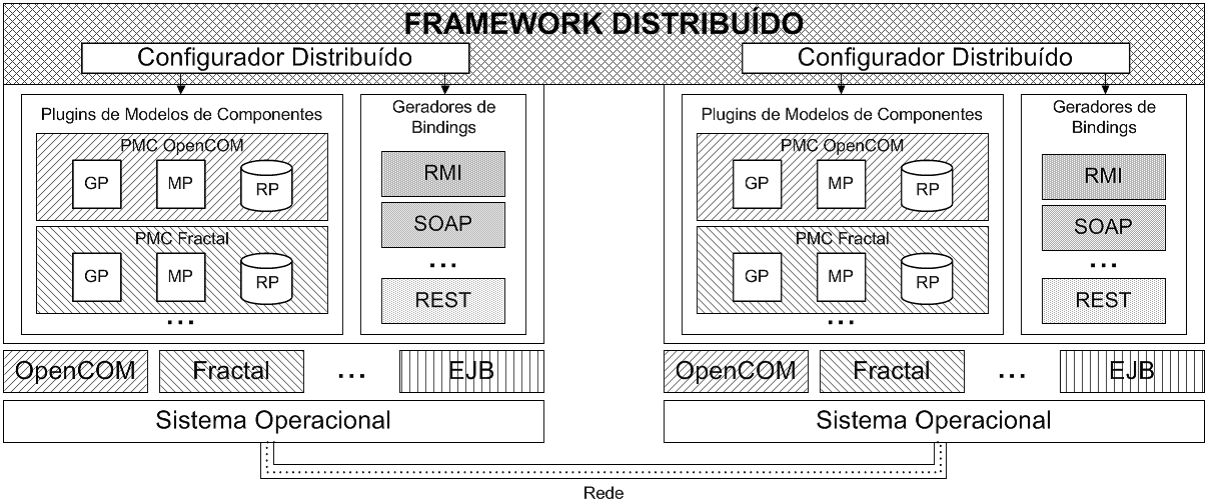
\includegraphics[scale=0.5]{figuras/010InteropArquitetura.png}
	\caption{Arquitetura do InteropFrame \cite{nascimento2013}.}
	\label{fig:010 - interop}
\end{figure}

A Figura \ref{fig:009 - interop02} mostra o funcionamento do InteropFrame. Neste cen�rio o usu�rio deseja interconectar os componentes ``A'' e ``B'', desenvolvidos respectivamente em OpenCOM e Fractal. O componente ``A'' � tratado aqui como componente cliente pois requisita os servi�os do componente servidor ``B'' de modo remoto.

O detalhamento deste processo de funcionamento para o exemplo da Figura \ref{fig:009 - interop02} � descrito a seguir \cite{nascimento2013}:

- Do lado do componente cliente
\begin{itemize}
	\item (1C) O Configurador Distribu�do (CD) verifica se o \textit{proxy} do lado cliente, necess�rio para promover a interoperabilidade, j� se encontra no Reposit�rio de \textit{Proxies} (RP), caso contr�rio ele solicita a gera��o do mesmo no passo 2C. Caso o componente \textit{proxy} j� exista, o pr�ximo passo ser� o 5C, onde esse componente ser� utilizado pelo Montador de \textit{Proxies} (MP);

	\item (2C) O CD solicita ao subm�dulo Gerador de \textit{Proxies} (GP) do modelo de componentes OpenCOM para gerar automaticamente o c�digo do componente ``X'' que representa o \textit{proxy} do lado cliente;

	\item (3C) O GP solicita ao subm�dulo Gerador de \textit{Bindings} (GB) do RMI para gerar automaticamente a parte do c�digo do componente ``X'' respons�vel pela comunica��o remota;

	\item (4C) O GP armazena no RP o componente ``X'' gerado;

	\item (5C) O CD solicita ao MP que proceda com a inicializa��o do \textit{proxy} do lado cliente;

	\item (6C) O MP obt�m e inicializa o componente ``X'' do lado cliente no ambiente de execu��o OpenCOM conectando o recept�culo do componente ``A'' � interface provida do \textit{proxy} ``X''. O \textit{proxy} ``X'' do lado cliente representa o componente ``B'' no lado cliente e tem seus servi�os requisitados pelo componente ``A''.
\end{itemize}

- Do lado do componente servidor
\begin{itemize}
	\item (1S) O Configurador Distribu�do (CD) verifica se o \textit{proxy} do lado servidor j� se encontra no Reposit�rio de \textit{Proxies} (RP), caso contr�rio ele solicita a gera��o do mesmo no passo 2S. Caso o componente \textit{proxy} j� exista, o pr�ximo passo ser� o 5S, onde esse componente ser� utilizado pelo Montador de \textit{Proxies} (MP);

	\item (2S) O CD solicita ao subm�dulo GP do modelo de componentes Fractal para gerar automaticamente o c�digo do componente ``Y'' que representa o \textit{proxy} (tamb�m chamado de \textit{skeleton}) do lado servidor;

	\item (3S) O GP solicita ao subm�dulo GB do RMI para gerar automaticamente a parte do c�digo do componente ``Y'' respons�vel pela comunica��o remota;

	\item (4S) O GP armazena no RP o componente ``Y'' gerado;

	\item (5S) O CD solicita ao MP que proceda com a inicializa��o do \textit{proxy} do lado servidor;

	\item (6S) O MP obt�m e inicializa o componente ``Y'' do lado servidor no ambiente de execu��o Fractal conectando o recept�culo do \textit{proxy} ``Y'' � interface provida do componente ``B''. O \textit{proxy} ``Y'' do lado servidor representa o componente ``A'' no lado servidor que requisita os servi�os do componente ``B''.
\end{itemize}

\begin{figure}[!h]
	\centering
		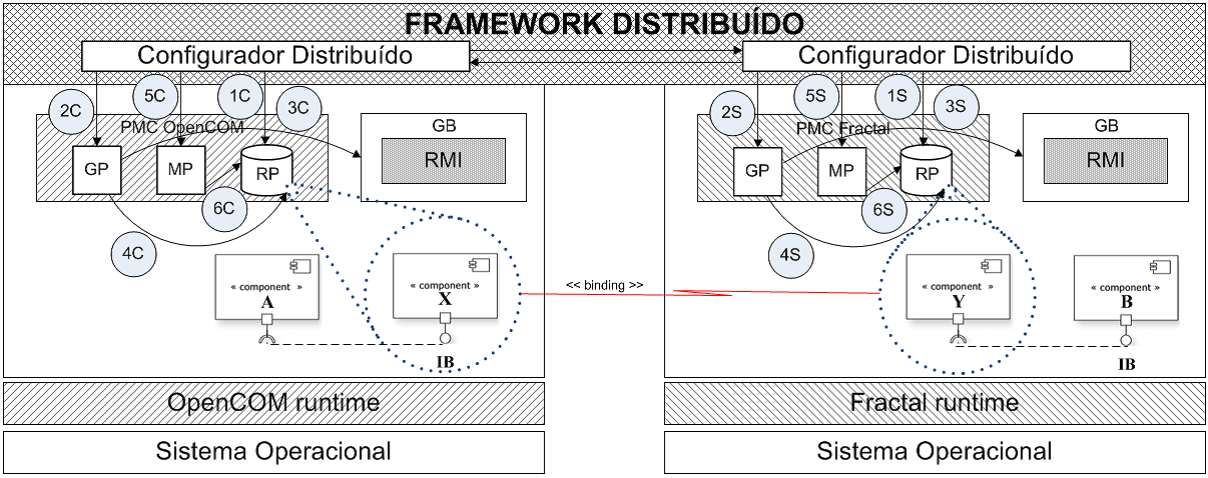
\includegraphics[scale=0.5]{figuras/009Interop02.png}
	\caption{Funcionamento do InteropFrame \cite{nascimento2013}.}
	\label{fig:009 - interop02}
\end{figure}

Com o \textit{binding} executado, o componente ``A'' agora pode utilizar os servi�os do componente ``B'' de forma transparente. Quando uma requisi��o � feita no componente ``A'' ela � repassada via RMI do componente \textit{proxy} ``X'' para o componente \textit{skeleton} ``Y'' e este por sua vez repassa para o componente ``B''. A resposta dessa requisi��o � feita pelo caminho inverso, de ``B'' para ``Y'', de ``Y'' para ``X'' e de ``X'' para ``A''. Na pr�tica, ``A'' e ``X'' s�o componentes do modelo OpenCOM, assim como ``B'' e ``Y'' s�o do modelo Fractal. Os componentes ``X'' e ``Y'' se comunicam atrav�s de RMI, garantindo assim a interoperabilidade entre os componentes ``A'' e ``B''.

\section{Modulariza��o do InteropFrame}

O InteropFrame foi desenvolvido em Java ``puro'', de forma a permitir a extensibilidade para novos modelos de componentes e de \textit{bindings}. Cada \textit{plug-in} de modelo de componentes ou de \textit{binding} fornece o suporte a um modelo de componentes ou de \textit{binding} espec�fico. Com o desenvolvimento de novos \textit{plug-ins} a ferramenta passa a suportar novos modelos.

Segundo \citeonline{hall2011} o Java prov� alguns aspectos de modulariza��o atrav�s da orienta��o a objetos, por�m n�o foi proposto para suportar modulariza��o de alta granularidade. {hall2011} ainda cita algumas limita��es do Java no quesito modulariza��o:
\begin{itemize}
	\item Baixo n�vel de controle de visibilidade de c�digo: Os modificadores de acesso do Java (\textit{public, protected e private}) tratam em baixo n�vel o encapsulamento da orienta��o a objetos e n�o no n�vel de particionamento l�gico do sistema. Em Java, um \textit{package} (pacote) � tipicamente utilizado para particionar c�digo. Para este c�digo ser vis�vel por um outro \textit{package}, ele deve ser declarado como \textit{public}. Algumas vezes, a estrutura l�gica da aplica��o faz chamadas a c�digos de \textit{packages} diferentes, significando que qualquer depend�ncia entre os pacotes deve ser exposta como \textit{public}. Dessa maneira, os detalhes de implementa��o tornam-se p�blicos, dificultando a evolu��o do sistema devido a poss�vel cria��o de depend�ncias da API n�o p�blica.
	\item Conceito de \textit{Classpath} propenso a erros: Aplica��es s�o compostas de v�rias vers�es de bibliotecas e componentes. O \textit{Classpath} do Java n�o lida com vers�es de c�digo, retornando assim o primeiro que encontra. O modo de constru��o do \textit{Classpath} n�o permite especificar vers�es de um mesmo c�digo. Em Java apenas se vai colocando as bibliotecas (comumente arquivos JAR) at� que a JVM (Java Virtual Machine) pare de acusar erros sobre classes faltantes.
	\item Implanta��o limitada e suporte a gerenciamento: N�o h� maneira f�cil em Java de se implantar um conjunto particular de depend�ncias de c�digo versionadas e executar a aplica��o. Tamb�m � dificultada a evolu��o da aplica��o e seus componentes ap�s a implanta��o. O Java n�o possui um suporte direto � cria��o de \textit{plug-ins} din�micos, o que � conseguido apenas atrav�s do uso de \textit{Class Loaders} - mecanismos de baixo n�vel e propensos a erros.
\end{itemize}

\begin{figure}[!h]
	\centering
		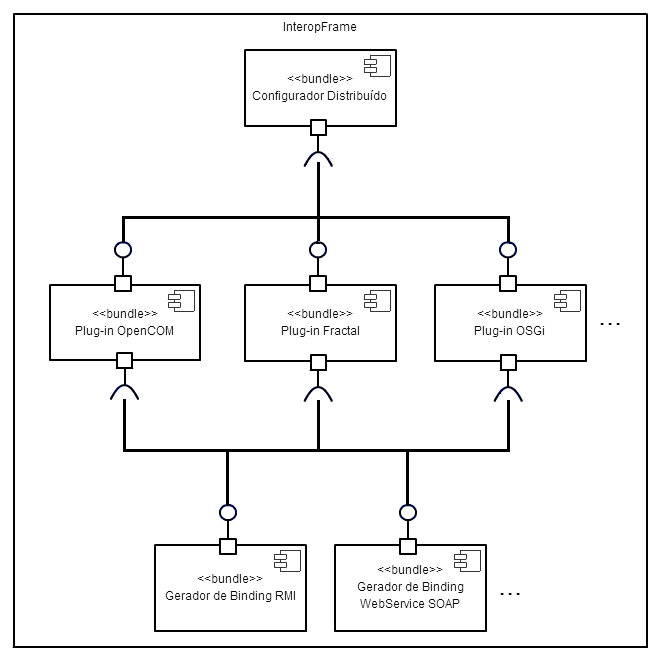
\includegraphics[scale=0.7]{figuras/008Interop.png}
	\caption{Bundles do InteropFrame em OSGi}
	\label{fig:008 - interop}
\end{figure}

Tendo em vista as limita��es do Java, necessita-se de uma maneira mais eficiente para a modulariza��o do InteropFrame. A proposta deste trabalho consiste na ado��o do OSGi como plataforma de modulariza��o. A extensibilidade do InteropFrame passar� a ter um suporte facilitado, uma vez que a aplica��o ser� desenvolvida em \textit{bundles} independentes como mostra a Figura \ref{fig:008 - interop}. Cada \textit{Plug-in} de Modelo de Componente e seus respectivos subm�dulos seriam portados para \textit{bundles} OSGi individuais. Da mesma forma, cada Gerador de \textit{Binding} tamb�m se tornaria um \textit{bundle} independente, bem como o n�cleo do InteropFrame e o Configurador Distribu�do.

\section{Solu��o de comunica��o do Configurador Distribu�do}

O Configurador Distribu�do, m�dulo respons�vel pelo gerenciamento entre as partes distribu�das do InteropFrame, � desenvolvido utilizando a tecnologia Java RMI. O Configurador Distribu�do atua na comunica��o remota entre os lados servidor e cliente do InteropFrame. O lado servidor � respons�vel por propagar pela rede uma interface provida de um componente de um dado sistema. O lado cliente faz a utiliza��o desse servi�o fornecido pelo lado servidor.

Para garantir uma comunica��o distribu�da de forma modular, este trabalho prop�e a ado��o da comunica��o remota baseada no ECF (\textit{Eclipse Communication Framework}) para a implementa��o do Configurador Distribu�do. O ECF consiste num conjunto \textit{frameworks} para a constru��o de servidores distribu�dos e aplica��es. Prov� implementa��o modular do padr�o de servi�os remotos do OSGi, juntamente ao suporte para \textit{Web Services REST} \cite{ecf2014}.

\section{Extens�o para o modelo de componentes OSGi}

Al�m da modulariza��o utilizando o OSGi, tamb�m � proposto neste trabalho a extens�o para o suporte ao modelo de componentes OSGi dentro do InteropFrame.

Ap�s a portabilidade do InteropFrame para a plataforma OSGi, ser� criado um novo \textit{plug-in} para que o \textit{framework} passe a suportar o OSGi como um modelo de componentes interoper�vel com os j� existentes (OpenCOM e Fractal). Essa proposta tem como objetivo avaliar o processo de desenvolvimento de um novo \textit{plug-in} de modelo de componentes.


\chapter{Considera��es Finais}\label{chap:consideracoes}

O InteropFrame � uma solu��o que auxilia na resolu��o de problemas relacionados � interoperabilidade entre componentes distribu�dos de modelos heterog�neos. Por�m, essa solu��o est� apenas limitada aos modelos OpenCOM e Fractal, al�m de promover a comunica��o remota apenas utilizando Java RMI ou \textit{Web Service SOAP}. Outra limita��o � que o InteropFrame foi desenvolvido em Java ``puro'', o que dificulta a sua extensibilidade. Outro problema do InteropFrame � a sua comunica��o interna (entre os lados cliente e servidor), que � feita atrav�s de Java RMI.

Este trabalho prop�e uma poss�vel solu��o para essa limita��o atrav�s da utiliza��o do OSGi como forma de modularizar o InteropFrame, al�m da extens�o para o OSGi como um modelo de componentes interoper�vel dentro da ferramenta. Tamb�m prop�e a resolu��o dos problemas relacionados � comunica��o interna atrav�s dos mecanismos de comunica��o providos pelo \textit{Eclipse Communication Framework}. Dessa forma, o InteropFrame torna-se mais extens�vel, coeso e desacoplado.
% ----------------------------------------------------------
% Introdução (exemplo de capítulo sem numeração, mas presente no Sumário)
% ----------------------------------------------------------
%\chapter*[Introdução]{Introdução}
%\addcontentsline{toc}{chapter}{Introdução}
% ----------------------------------------------------------



% ----------------------------------------------------------
% ELEMENTOS PÓS-TEXTUAIS
% ----------------------------------------------------------
\postextual
% ----------------------------------------------------------

% ----------------------------------------------------------
% Referências bibliográficas
% ----------------------------------------------------------
\bibliography{referencias}

% ----------------------------------------------------------
% Glossário
% ----------------------------------------------------------
%
% Consulte o manual da classe abntex2 para orientações sobre o glossário.
%
%\glossary

% ----------------------------------------------------------
% Apêndices
% ----------------------------------------------------------

% ---
% Inicia os apêndices
% ---

% ---


% ----------------------------------------------------------
% Anexos
% ----------------------------------------------------------

% ---
% Inicia os anexos
% ---


%---------------------------------------------------------------------
% INDICE REMISSIVO
%---------------------------------------------------------------------

%---------------------------------------------------------------------

\end{document}
